\newpage

\section{Remerciements}\label{remerciements}

\bigskip

Je tiens à remercier Benjamin Tierny, Robin Komiwes et Julien Vanden
Torren de m'avoir acceuilli chez Dernier cri pour mon stage.

\bigskip

Je remercie également mon suiveur Harry Claisse pour son aide et son
accompagnement, ainsi que les enseignants de l'Université technologique
de Compiègne.

\bigskip

Merci également à toute l'équipe de Dernier cri pour avoir rendu mon
stage si enrichissant et agréable.

\newpage

\section{Introduction}\label{introduction}

\bigskip

Dans le cadre de mon TN09 à l'Université technologique de Compiègne,
j'ai effectué un stage de six mois chez Dernier cri.

\bigskip

Dernier Cri est une Start-Up crée en 2011 spécialisé dans l'innovation
numérique. L'équipe est en charge du développement, du déploiement et de
la maintenance d'applications pour le compte de plusieurs clients.

\bigskip

Ma mission à été d'intégrer l'équipe de developpement pour aider dans la
création de plusieurs applications web.

\bigskip

J'ai pus lors de ce stage intégrer une équipe dynamique etpro-active.
J'ai notamment pus prendre part à de nombreuses présentations internes
sur différentes technologies, à l'écriture d'article de blog. J'ai
également pus participer activement à la relation cliente lors de mes
projets.

\newpage

\section{Dernier cri}\label{dernier-cri}

\bigskip

\subsection{Histoire}\label{histoire}

\bigskip

En 2011 Robin Komiwes et Benjamin Tierny créent Nectify dans le but de
développer \textbf{Fresc}, un outil de partage d'avis sur des visuels.
Bien que cet outil connait un succés certain avec aujourd'hui plus de
300 sociétés utilisant Fresc à travers des milliers de projets, la
rentabilité du projet n'est pas suffisante.

\bigskip

Nectify choisi alors de compléter ses revenus par de la prestation de
services centrée sur l'innovation.

\bigskip

Début 2014, la majeure partie du chiffre d'affaire de Nectify était dû
aux activités de prestations de services, Fresc ne représentant qu'une
part marginale.

\bigskip

Devenant donc une agence spécialisée dans l'innovation digitale, Nectify
choisi de changer de créé sa propre image, distincte de Fresc. C'est
dans se mouvement que la société est devenu \textbf{Dernier cri}.

\bigskip

Aujourd'hui \textbf{Dernier cri} est une agence web

(Dernier Cri met un point d'honneur à proposer à ses clients une
solution complète adaptée à un problème spécifique. De la conception à
la réalisation, l'entreprise accompagne ses clients de A à Z pour
aboutir à un produit au plus proche des besoins de ceux-ci. Cela permet
aux développeurs d'opérer dans différents domaines d'activités et
d'avoir une vue globale du développement de produit.)

\bigskip

\begin{figure}
\centering
\includegraphics{logo_DC}
\caption{logo}
\end{figure}

\newpage

\subsection{Secteur d'activité}\label{secteur-dactivituxe9}

\bigskip

\subsection{Organisation}\label{organisation}

\bigskip

L'entreprise est constitué de 16 employés. Le CEO de l'entreprise est
Benjamin Tierny, co-fondateur de Dernier cri, tandis que Robin Komiwes
est CTO.

\bigskip

Le troisième associé, Julien Vanden Torren, est Account Manager. C'est à
dire le lien entre l'entreprise et les clients.

\bigskip

L'entreprise est également constitué d'une chef de projet, Laetitia
Cocusse, qui s'occupe de superviser la pluspars des projet.

\bigskip

L'équipe de développeur est constitué notament d'un devops, c'est à dire
possédant à la fois les compétences d'un développeur et d'un ingénieur
système (Jean-Serge Monbailly), d'un Data Scientist (Antonin Carette)
qui travaille sur les projet de big data.

\bigskip

La plupars des développeurs travails sur plusieurs projets en même
temps, selon les besoins de l'entreprise et les compétences de chacun.
Des équipes de 2/3 developpeurs sont créé, mélangeant les compétences
front et back, de developpement et de systeme.

\bigskip

\begin{figure}
\centering
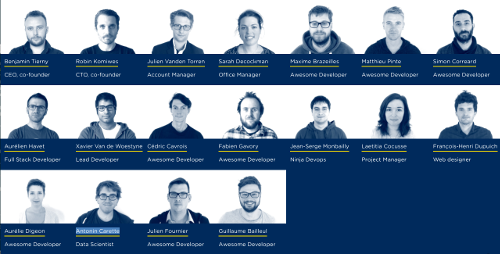
\includegraphics{team.png}
\caption{image}
\end{figure}

\subsubsection{Github et code review}\label{github-et-code-review}

\bigskip

L'entreprise utilise principalement la plateforme Github comme service
web d'hébergement et donc le logiciel de gestion de versions Git. Github
permet au developpeur de travailler à plusieurs sur le même projet, de
résoudre rapidement des conflits dus à la modification d'un même
document pars plusieurs personne, de gérer différente version du projet
etc\ldots{}

\bigskip

Une nouvelle version de Githib propose une section \textbf{Projet}
permttant de gérer les \textbf{issues}, c'est à dire les taches. Cette
section permet de notamment de séparer les taches en plusieur colonnes,
par exemple : \emph{A faire}, \emph{En cours}, \emph{Terminé}. Il est
aussi possible d'attribuer les taches à un contributeur, ou encore de
leur attribuer des labels tel que \emph{Urgent}, \emph{Bug} ou encore
une estimation de temps quand à la réalisation de la tache.

\bigskip

Dernier cri utilisait jusque la un outil similaire. Il a été décidé
d'utiliser la section \textbf{Projet} de Github pour les nouveaux
projets, notamment ceux sur lesquels j'ai étais affecté.

\bigskip

Github offre aussi un outils de \emph{Code Review}, c'est à dire de
relecture du code avant son incoration au projet. Dernier cri utilise ce
systéme pour garantir une certaine qualité du code ainsi qu'un style
d'écriture homogéne. C'est également l'occasion pour les développeurs

\bigskip

Dernier cri à mis en place un processus de vérification de la qualités
du code et d'entraide. Chaque developpeur, une fois une tache terminé,
propose une \emph{Pull request}, c'est à dire demande à fussionner sa
version du projet, modifié pour résoudre la tache, avec la version
principal, stable. Il demande ensuite à ses collégues ayant des
compétences dans le langage utilisé de relire et de commenter cette
\emph{Pull request}.

\bigskip

Ce processus permet non seulement de garantir la qualité du code mais
permet aussi de proposer des solution, des syntaxes alternatives, que
peut être le developpeur ne connaissait pas. Bien souvent c'est aussi
l'occassion de débatre sur le bien fondé d'habitudes, ou de conventions.

\bigskip

\subsubsection{Talk interne}\label{talk-interne}

\bigskip

Dans l'optique du partage du savoir dans l'entreprise, les employés sont
invités à faire des présentation en interne. Les présentation peuvent
autant porter sur des langages de programmation, des nouvelles
technologies, de la gestion de projet \ldots{}

\bigskip

Cela permet d'interresser les autres sur certain sujets, de partager ses
connaissances. Pour la personne organisant la conférences c'est aussi
une occasion de

\bigskip

Durant mon stage j'ai eu l'occasion d'assister à des présentation sur
React, Docker, Rust, MJML

\bigskip

Ces présentations sont publiées sur la
\href{https://www.youtube.com/channel/UCDfdBlzldhg_PEu3xZTPsHg}{chaîne
youtube Dernier cri}

\bigskip

\subsubsection{Article de blog}\label{article-de-blog}

\bigskip

\bigskip

\subsection{Take off conf}\label{take-off-conf}

\bigskip

\bigskip

\newpage

\section{Cadre du stage}\label{cadre-du-stage}

\bigskip

-\textgreater{} Relation clients -\textgreater{} Mise en production

Durant mon stage j'ai pus participer au développement de deux
applications. Ces deux projets s'appuyé sur du React, une bibliothèque
JavaScript libre développée par Facebook depuis 2013. N'ayant jamais
utilisé cette bibliothéque, j'ai donc du tout d'abord me former.

\bigskip

Le premier projet auquel j'ai participé se nomme Photolix. C'est un site
internet de développement de photos, avec pour objectifs de toucher un
public \ldots{}. et de limiter au maximum le temps d'attente du client
en envoyant les photos au serveur dès leur sélection.

\bigskip

Le second projet est FinFrog, un site proposant des prêts financés par
des particuliers. Ce projet était déjà assez avancé à mon arrivé. Le
client possédait un site en ligne, mais souhaité changer l'apparence et
ajouter des fonctionnalités, ce pourquoi il a fait appel à Dernier cri.

\subsection{Formation}\label{formation}

\bigskip

Lors de mon arrivée chez Dernier cri, j'ai eu l'occasion de me former
sur Javascript ES6, React ainsi que Redux, car l'entreprise prévoyé de
me mettre sur des projets utilisant ces technologie.

\bigskip

Ces trois technologie étant \ldots{} (ca m'intéresse et en plus c'est
hype)

\bigskip

Ma formation c'est faite à partir du site https://www.codeschool.com/,
disposant de cours en vidéos ainsi que d'exercices intéractifs.

\bigskip

\subsubsection{Javascript ES6}\label{javascript-es6}

\bigskip

Le Javascript est un langage de programmation de scripts incourtounable
du web. Si à sa création il servait principalement à la réalisation
d'animation, il est aujourd'hui au centre des applications. Le javacript
sert maintenant à controler presque la totalité de l'application web.
Cependant, ce langage n'étant pas était prévu pour une telle compléxité,
il en résulte une syntaxe complexe et lourde. C'est dans ce contexte
qu'un mise à jour du langage c'est imposé.

\bigskip

ES6 (ECMAScript Edition 6 ou encore ES2015) a été publiée en juin 2015.
Il ajoute un ensemble de normes a celles déja présente pour apporter de
nouvelle fonctionnalités qui permettent d'alléger le code, de le
structurer, et de le rendre notamment plus maintenables, tout en restant
compatibles avec le code existant.

\bigskip

ES6 n'est pas encore totalement supporté par les navigateurs, il est
donc utilise d'utiliser un transcompilateur vers ES5, comme Babel.js.

\bigskip

L'apprentissage de ES6 a était primordiale pour mon stage : les
nouvelles normes rende vraiment le code plus facile à lire et à écrire.
J'ai eu l'occasion durant mon stage de travailler sur un projet
JavaScript n'utilisant pas ES6 et j'ai eu de grande difficultés à me
passer des facilité d'écritures.

\bigskip

\subsubsection{React}\label{react}

\bigskip

Developpé depuis 2013 par Facebook, React est une bibliothèque
JavaScript déclarative, efficace et flexible pour la création
d'interfaces utilisateur. Cette bibliothéque c'est démarqué notamment
par ses performances.

\bigskip

Elle est aujourd'hui utilisé par de nombreuses entreprises tel que
Netflix, Yahoo, Airbnb ou encore Sony.

\bigskip

Une des particulariés de React est de découper l'application en
composants, dépendant d'un état. Lors du changement de l'état d'un
composant, React génére les changements en HTML pour les répercutés sur
la page. Grace à l'utilisation d'un DOM virtuel, c'est à dire d'une
représentation de la vue, React fait le minimum de modification
possible, ce qui explique ces performances.

\bigskip

Cette bibliothéque est aujourd'hui en expensions. Elle a un succés
certain auprès de la communautés des developpeurs web, et de nombreux
outils se developpe autours. C'est donc un avantage certain d'avoir pu
apprendre React lors de mon stage, puis d'avoir mis en pratique ces
connaissances lors des deux projets que j'ai effectués.

\bigskip

\subsubsection{Redux}\label{redux}

\subsection{gestion de projet}\label{gestion-de-projet}

-\textgreater{} Expliquer le déroulement : laetitia qui parle au client
pour saoir ses besoin, qui crée l'issu, etc\ldots{}

\subsection{Photolix}\label{photolix}

\subsubsection{Présentation du projet}\label{pruxe9sentation-du-projet}

\subsubsection{Objectifs}\label{objectifs}

\subsubsection{Déroulement}\label{duxe9roulement}

\subsubsection{Difficultés}\label{difficultuxe9s}

\subsubsection{Conclusion}\label{conclusion}

\subsection{Finfrog}\label{finfrog}

\subsubsection{Présentation du
projet}\label{pruxe9sentation-du-projet-1}

\subsubsection{Nouveaux outils}\label{nouveaux-outils}

\subsubsection{Organisation}\label{organisation-1}

\subsubsection{Difficultés}\label{difficultuxe9s-1}

\section{Conclusion}\label{conclusion-1}

-\textgreater{} Compétences apprises : React Redux ES6 Relation client
Git Github pm2 npm

-\textgreater{} environnement cool : Ambiance, tech off conf , meetup
